\section{Grundlagen}
\begin{frame}{}
    \begin{center}
        Grundlagen
     \end{center}
\end{frame}

\begin{frame}{Ein typisches Freifunk Netz}
    \begin{itemize}
        \item Ein Batman-Adv Netz
        \begin{itemize}
            \item[$\rightarrow$] "Wie ein großer dezentraler Switch"
        \end{itemize}
        \item VPN für die Funkinseln
        \begin{itemize}
            \item Multi-Client zu Multi-Client VPN
            \item Layer-II Netz
            \item Kein internes Routing / Forwarding
        \end{itemize}
        \item Mehrere VPN Server / Gateway
        \begin{itemize}
            \item DHCP
            \item DNS Namensauflösung
            \item Gateway zum Internet / ICVPN
        \end{itemize}
        \item Monitoring
        \begin{itemize}
            \item Karte aller Knoten
        \end{itemize}
    \end{itemize}
\end{frame}

\begin{frame}{Ein typisches Freifunk Netz}
    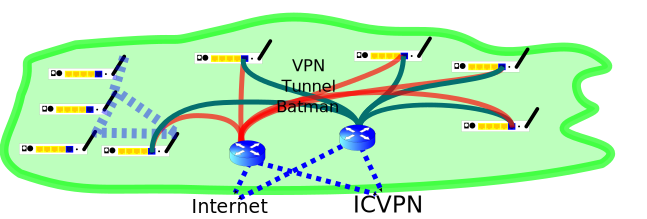
\includegraphics[width=\textwidth]{img/svg/freifunk_konzepte_alt.pdf}
\end{frame}

\begin{frame}{Freifunk Franken Netz}
    \includegraphics[width=\textwidth]{img/svg/freifunk_konzepte.pdf}

    \begin{itemize}
        \item Mehrere Layer-2 Inseln (Hoods)
        \item Verbindung per Layer-3
        \item Dezentrale Gateways
    \end{itemize}
\end{frame}

\begin{frame}{Knoten VPN}
    \begin{itemize}
        \item Verwendetes VPN: fastd
        \begin{itemize}
            \item n:m VPN
        \end{itemize}
        \item Endpunkt Vermittlung über KeyXchange:
        \begin{itemize}
            \item Zentrale Webseite \only<2-3>{{\color{red}Problem!}}
            \item Knoten meldet sich mit Standort
            \item Geographisch nächste Hood wird zugewiesen (voronoi)
            \item Client bekommt Liste aller Server der Hood
        \end{itemize}
        \item<3> Keine weitere Unterscheidung zu welcher Hood der Knoten gehört
        \item<3> {\color{red}Problem!} Funk Verbindung zwischen den Hoods
    \end{itemize}
\end{frame}

\begin{frame}{VPN Server}
    \begin{itemize}
        \item VPN Server: In jeder Hood gibt es mehrere davon
        \item Hoodzuweisung manuell im KeyXchange
        \item DHCP
        \begin{itemize}
            \item Aktuell ausschließlich IPv4
            \item Unterschiedliche Latenzen: Ungleiche Server Auslastung
            \begin{itemize}
                \item[$\rightarrow$] Batman-Adv GW Selection
                \item Anpassung nach Traffic Auslastung
            \end{itemize}
        \end{itemize}
        \item DNS Namesauflösung
        \item Policy base routing
        \item VPN (GRE) Tunnel zu anderen Gateways
        \begin{itemize}
            \item OLSR Routing
        \end{itemize}
    \end{itemize}
\end{frame}

\begin{frame}{Gateways}
    \begin{itemize}
        \item Verbindet Freifunk und Internet
        \item IPv4 NAT (oft übers Ausland) ins Internet
        \item Announced 0.0.0.0/0 via OLSR
        \begin{itemize}
            \item Dynamic Gateway Plugin
            \item VPN Server können diese Routen nutzen
        \end{itemize}
        \item Routing Metrik ohne Traffic/Bandbreite
        \item<2> {\color{red}Problem!} Ungleiche Traffic Verteilung
    \end{itemize}
\end{frame}
